\chapter{仿冒应用的评论分析}
\label{chp:feedback}

应用市场中的用户反馈区是Android应用生态的重要部分,也是移动黑灰产从业者的深耕之地。
热心用户会在评论区提出反馈,黑灰产从业者则会利用排名欺诈的手段牟取利益。
为了进一步对仿冒应用的生态有所了解,作者有必要搜集和分析仿冒应用的评论。
对于与仿冒应用相关的评论,有以下待解答的问题:
有多少用户会对这些应用进行评论?
用户对这些应用的使用感受如何?
仿冒应用是否会跟排名欺诈有所联系?

为了回答这些问题,作者从\texttt{360手机助手}应用商店中爬取了部分应用和它们的所有历史评论,然后对这些评论进行了处理和分析。

\section{仿冒评论数据收集}
由于Janus平台上并不提供评论数据,所以作者重新在应用市场上收集评论数据。
在\texttt{360手机助手}应用商店中,作者随机挑选了856个应用,爬取了这些应用的APK包和它们的所有历史评论。
之后,作者将上一次数据收集时保存的正版应用的信息重新导入\mytool,并从这一批应用中筛选出了对应仿冒应用。

每条评论都会附带一个评价分数,某款App在市场上的平均评价就是所有评论评分的均值。
对于每条评论信息,作者能收集到的数据项是:\texttt{应用包名}、\texttt{用户ID}、\texttt{评论内容}、\texttt{评分}和\texttt{评论日期}共五项。

\subsection{评论数据概览}
在作者收集评论的所有856个应用中,有6款应用与先前仿冒应用数据中的包名对应。
要注意的是,由于本研究的仿冒应用列表为针对50个热度最高的目标App整理而成,而收集评论的应用是在整个市场范围内随机挑选的,所以这里的仿冒应用占总体应用比例较小。但这不意味着整个市场中就只有这几款应用是仿冒应用。
另外,由于这856个应用是随机挑选的,作者认为这批数据具有一定的代表性,可以应以反映整个市场的评论分布情况。
本次研究一共爬取到了267,397名用户的365,461条评论,其中6款仿冒应用的所有历史评论共计3,591条,来自2,946名用户。

\subsection{基础分析}

% 画图用的python代码
% font_size = 20
% sns.set(style="white")
% fig = plt.figure()
% plt.xticks(fontsize=20)
%
% ax1 = fig.add_subplot(111)
% bar = sns.barplot(x="Package name", y="Comment cnt", data=df, ax=ax1, palette="Blues_r")
% ax1.tick_params(axis='y', labelcolor=“tab:blue”)
% plt.yticks(fontsize=font_size)
% ax1.set_ylabel("# Comments", color="tab:blue", size=font_size)
%
% ax2 = ax1.twinx()
% line = sns.lineplot(x="Package name", y="Rating", data=df, ax=ax2, c="r", linewidth=3)
% ax2.tick_params(axis='y', labelcolor=“tab:red”)
% ax2.set_ylabel("Rating", color="tab:red", size=font_size)
% plt.yticks(fontsize=font_size)
% # 折线图y轴范围
% plt.setp(line, yticks=[4, 4.2, 4.4, 4.6, 4.8])
% # 旋转x轴标签
% for axis in [ax1, ax2]:
%     for tick in axis.get_xticklabels():
%         tick.set_rotation(10)
%
% # 清除上方右方边框
% sns.despine()
% plt.show()

\begin{figure}[htbp]
	\centering
	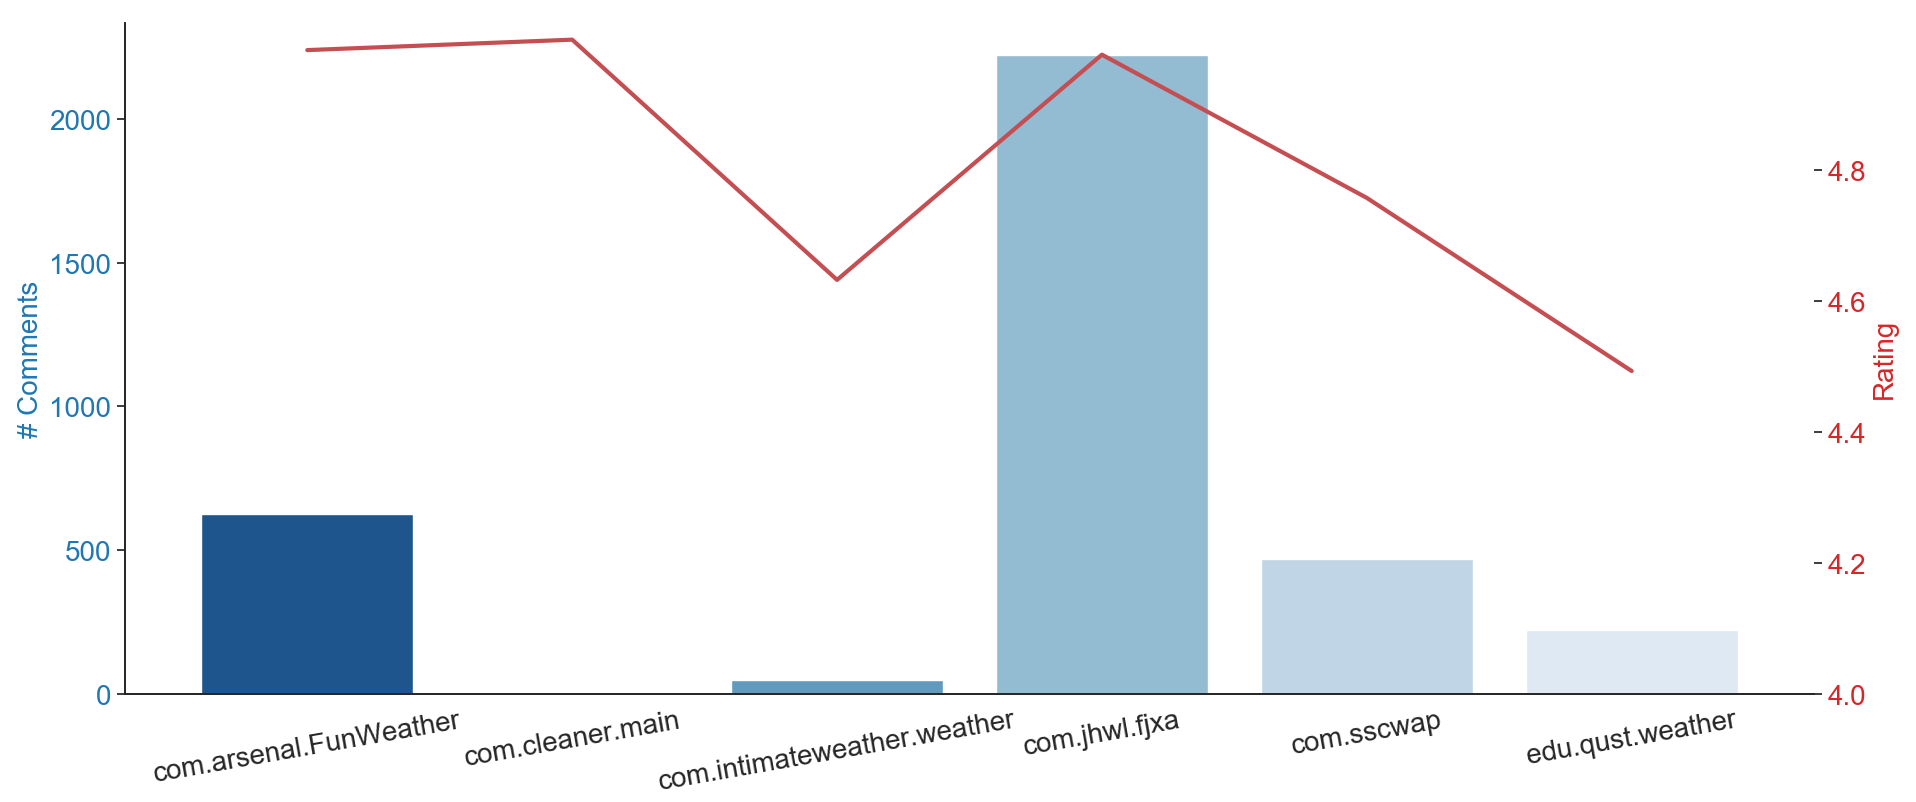
\includegraphics[width=\textwidth]{./Figures/edwin-cmt-ratings-dist-3.png}
    \caption{各仿冒应用在\texttt{360手机助手}商店中的评论数量与评分分布}
    \label{fig:cmt_dist_fake}
\end{figure}

\autoref{fig:cmt_dist_fake}显示了6款应用收到的评论数量和评分分布。
蓝色的柱状图表示评论数量,红色的折线图表示各评论汇总后的平均评分(以5分为满分算),$x$轴分别代表不同样本的包名。
按评论数从多到少的顺序看,\emph{com.jhwl.fjxa}收到了2223条评论,平均评价为4.98分;
\emph{com.arsenal.FunWeather}收到了626条评论,平均评价也是4.98分;
\emph{com.sscwap}收到了467条评论,平均评价4.76分;
\emph{edu.qust.weather}收到了223条评论,平均评价4.49;
\emph{com.intimateweather.weather}和\emph{com.cleaner.main}分别只收到了49条和3条评论,而他们的平均评价则分别为4.63分和5分。
乍眼一看,上述应用的评分都十分高。
以下是一些热门应用的评分和这些仿冒应用的评分的对比:
在同一市场下,移动购物类应用\texttt{淘宝}的评分为4.55分,近年十分受欢迎的短视频应用\texttt{抖音}平均评价是4.5分,游戏类应用\texttt{开心消消乐}的评分是3.65分,而\texttt{微信}的平均评价更是只有3.45分。
上述应用毫无疑问都是十分优质的App,庞大的用户基数带来的大量真实评价会使得平均评价较为稳定,不会因为在短时间内收到少量好评或者差评就产生较大的评价波动。
在\texttt{淘宝}等应用作为基准的情况下,6款仿冒应用的评分之高不禁令作者想到恶意刷评的相关研究。
但本研究不能仅凭几个应用的平均评价对比就咬定仿冒应用存在刷好评的行为,所以本文会应该先分析数据集的整体分布再作进一步比较。

在不考虑上述提到的恶意刷评的情况下,一款应用的使用人数越多,就越有可能收到来自用户的评价。
所以可以在一定程度上,从一款应用的评论数目估计其用户数量的多少。
\autoref{fig:cmt_dist_total}中的两个小提琴图显示了所有856个应用收到评论的数量和总体评级分布,这有助于让读者了解市场中应用的热度分布情况和用户的评价倾向。

% Python 作图代码
% font_size = 20
% sns.set(style="whitegrid")
% fig = plt.figure()
%
% ax1 = fig.add_subplot(121)
% bar = sns.violinplot(x=df2["Cmt cnt"], ax=ax1)
% ax1.set_xlabel("Package #Comment Distribution", size=20)
% plt.xticks(size=20)
%
% ax2 = fig.add_subplot(122)
% line = sns.violinplot(x=df2["Pkg Rating"], ax=ax2)
% ax2.set_xlabel("Package Rating Distribution", size=20)
% plt.xticks(size=20)
%
% # 清除上方右方边框
% sns.despine()
% plt.show()

\begin{figure}[htbp]
	\centering
	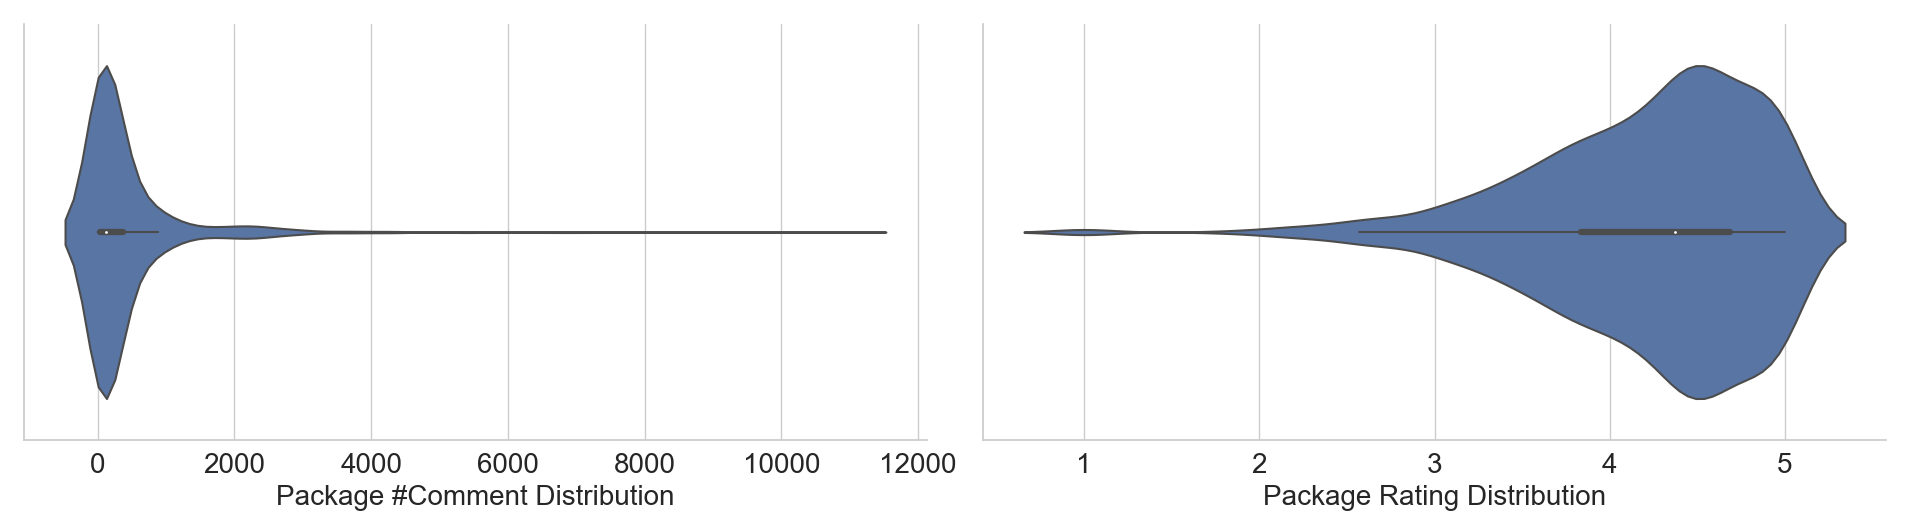
\includegraphics[width=\textwidth]{./Figures/edwin-360-comment-dist.png}
    \caption{所有856个应用在商店中的评论数量与评分分布}
    \label{fig:cmt_dist_total}
\end{figure}

左边的小提琴图表示每个应用收到的评论总数分布,其四分位数分别为31, 124和375.75。
这说明,在收集到的856个应用中,25\%的应用收到小于或者等于31条评论,50\%的应用收到小于或等于124条评论。
如果某款应用收到的评论数大于375条,那这款应用的评论总数就能排在前25\%了。
另外,数据显示,仅有5\%的应用收到了超过2,109条评论。
结合仿冒样本的数据,\emph{com.jhwl.fjxa}、\emph{com.arsenal.FunWeather}和\emph{com.sscwap}的评论数量都排在了前25\%,\emph{com.jhwl.fjxa}更是能排在前5\%的位置。
从数据上看,上面三款App相当受欢迎。

右边的小提琴图则表示各个应用收到的平均评价的分布情况,其四分位数分别为3.84,4.37和4.69,约5\%的应用平均评价为5分满分。
这个分布说明这个应用市场上的用户十分倾向于给出高分评价,至少有过半数的评论都是满分好评。
回到仿冒样本的数据,其中有两款评论少于100条,很可能存在较大的个体偏差,在此先忽略不计。
余下四款仿冒应用中也有三款的平均评价排进了前25\%,恰好也是评论数较多的\emph{com.jhwl.fjxa}、\emph{com.arsenal.FunWeather}和\emph{com.sscwap}。

结合两个维度的分布结果,\emph{com.jhwl.fjxa}、\emph{com.arsenal.FunWeather}、\emph{com.sscwap}三款App不仅用户众多,而且还好评如潮。
再回望\texttt{淘宝}、\texttt{微信}等应用的评分,两者之间似乎有了矛盾。
一款应用的用户越多,真实的评论数目越大,该款应用的评分就会趋向客观,直到收敛到一个可以反映应用质量的真实水平。
\emph{com.jhwl.fjxa}、\emph{com.arsenal.FunWeather}、\emph{com.sscwap}三款应用的用户量固然不能和\texttt{微信}、\texttt{淘宝}相比,但成百上千的评论数也暗示着一个不小的用户群体。
在用户群体有一定规模的情况下,还能保持名列前茅的平均评价,究竟是这三款仿冒应用的确受到了用户的热捧,还是另有原因?

\section{仿冒应用与排名欺诈关联验证}

\subsection{排名欺诈检测初探}

带着上述的疑问,作者决定用自动化的方法试图寻找这几款应用是否有排名欺诈的可能。

\texttt{FRAUDAR}~\cite{hooi2016fraudar}是Bryan Hooi在2016年推出的一个算法,可以使用二分图挖掘的方法找出可能的虚假好评,并输出最可能涉及排名欺诈的应用和用户。
算法基于的假设是,普通用户的行为(在本文中即为对App评论的行为)是大致随机的,而用于进行排名欺诈的用户群的行为却会有比较明显的指向性(即针对购买了排名欺诈服务的App发送好评),而且为了将平均评分拉高,就意味着需要发送大量好评。
如果将用户和App分别看做两种不同节点,每条好评看作是两种节点之间的边,那么在这张用户-评论-应用图中,排名欺诈用户和对应的App之间就会有特别紧密的联系。
如果能把这个联系特别紧密的子图找到,就有可能从中找到真实的排名欺诈用户和应用。

由于此处的排名欺诈指用大量虚假好评刷高应用的平均评价,所以在寻找排名欺诈用户和对应应用时,应该只采用满分好评作为数据。
因此,本研究从所有评论中筛选出了满分好评,其总数为381,507条,由229,100名用户给出,分布于848个应用中,占评论总数的87.15\%。
作者将\texttt{FRAUDAR}应用在了本研究的好评数据集上,找到了115名可疑用户和13个可疑应用。
经过比对后,作者发现,13个可疑应用并不包含仿冒样本,而仿冒应用的所有评论条目中也没有源于那115名可疑用户的评论。
但\emph{com.jhwl.fjxa}的评价表现依然令人生疑,因此,作者决定使用其他办法检测这几款仿冒应用的评论中是否存在排名欺诈的可能性。
基于本工作中现有的数据项,进行检测的角度可以分为两个,一个是评论用户可信度,另一个则是评论内容相似度。

\subsection{基于评论用户可信度的排名欺诈排查}

Mohammad-Ali~\cite{abbasi2013measuring}在2013年提出了一个个体行为相似度的计算方法。
在该算法中,用户行为相似度由\autoref{equ:usr_cre1}计算,如果相似度超过了某个阈值$T_1$,就可以将两名用户聚入同一类。
\autoref{equ:usr_cre1}中的$B(u_i, t)$指用户$u_i$在时间节点$t$的行为(在此处可以理解为对某一个应用给好评),而$\sigma(B(u_i, t), B(u_j, t))$则是一个用来计算用户$u_i$和$u_j$在时间为$t$时行为相似度的方程,Mohammad在文中选用的是\autoref{equ:usr_cre2}所示的Jaccard相似系数,所以本文在这里也选用了同样的Jaccard系数计算。

\begin{equation}
Sim(u_i, u_j) = \frac{1}{t_n - t_0}\sum_{t=t_0}^{t_n}\sigma(B(u_i, t), B(u_j, t))
\label{equ:usr_cre1}
\end{equation}
\begin{equation}
Jaccard(set_i, set_j) = \frac{|set_i \cap set_j|}{|set_i \cup set_j|}
\label{equ:usr_cre2}
\end{equation}
\vspace{0.5mm}

在这种计算方式下,那些仅给过一次好评的用户将会很容易成为噪声数据,对研究的结果产生影响,所以作者先剔除掉了这部分数据。
仅给过一次好评的用户共186,775人,占所有给出好评用户的81.53\%。

在将行为相似的用户聚类之后,可以通过计算某一应用评论中疑似排名欺诈评论的占比、或是评论该App的可疑用户占所有可疑用户的占比来排查可能购买了排名欺诈服务的App。

\begin{Def}
	应用的用户可信度权重

	假设所有市场用户的集合为$G_{all}$,已知疑似排名欺诈用户群体$G_r$,用户以$u$表示,由任意用户$u_i$发布的评论$cmt_j$表示为$u_i \rightarrow cmt_j$,市场中的某一应用$app_k$的评论列表为$CL_{app_k}$。
	则该应用$app_k$的用户可信度权重$W_{app_k}$可由\autoref{equ:usr_cre3}中的二元组表示:
\end{Def}

\begin{equation}
	W_{app_k} = (w_{app_k}^0, ~w_{app_k}^1)
	\label{equ:usr_cre3}
\end{equation}
\begin{equation}
	w_{app_k}^0 ~ = ~ \frac{|\{u_i~|~u_i \in G_r, cmt_j \rightarrow u_i, cmt_j \in CL_{app_k}\}|}{|G_r|}
	\label{equ:usr_cre4}
\end{equation}
\begin{equation}
	w_{app_k}^1 ~ = ~ \frac{|\{cmt_j~|~cmt_j \in CL_{app_k}, cmt_j \rightarrow u_i, u_i \in G_r\}|}{|CL_{app_k}|}
	\label{equ:usr_cre5}
\end{equation}
\vspace{0.5mm}

在计算完权重之后,可以分别按其中的两个子权重对应用进行排名,筛选出可能购买了排名欺诈服务的App。

作者分别将$T_1$设置为0.4,0.6和0.8,尝试对可疑用户进行聚类,结果分别将42,325名给出好评次数大于1的用户分到了10,024,14,520,15,493个聚类中。
可对这些聚类进行简单分析如下:
绝大多数聚类中都只有一名用户,即使是在相似度阈值只有0.4的情况下,也只有约7\%的聚类中包含3个或以上的用户(阈值为0.6和0.8时,该比例均为6\%)。
但是,当挑出包含用户数目大于10的聚类($T_1$为0.4/0.6/0.8时,这些聚类的占比分别为0.97\%/0.70\%/0.57\%)时,作者却发现这些聚类分别包含了29,168/23,742/22,218个用户,他们所发布的好评共计分别有98,226/80,492/73,422条。
因此作者推定,有一部分用户的行为模式相当近似且可疑,本文将会把这部分用户组成的群体看作是疑似的排名欺诈用户群体($G_r$)。

接下来,作者分别计算了不同$T_1$下,三款仿冒应用在\autoref{equ:usr_cre4}和\autoref{equ:usr_cre5}中的两个权重,即三款应用中的好评用户占可疑用户的比例、以及其好评占所有可疑用户发布的好评的比例。
对于本章研究的三个仿冒应用,其两个子权重的结果分别展示在\autoref{table:usr-cred-res-1}和\autoref{table:usr-cred-res-2}中。

\begin{table}[htbp]
	\renewcommand{\arraystretch}{1}
	\small
	\centering
	\caption{各应用用户可信度权重及对应排名(一)}
	\vspace{1mm}
	\begin{tabular}{lcccccc}
		\toprule
		包名 & $w^0$($T_1$=0.4) & 排名 & $w^0$($T_1$=0.6) & 排名 & $w^0$($T_1$=0.8) & 排名 \\
		\midrule
		com.arsenal.FunWeather & 0.97 & 2 & 0.9 & 6 & 0.82 & 9 \\
		\rowcolor{gray!15} com.jhwl.fjxa & 0.85 & 15 & 0.84 & 12 & 0.8 & 12 \\
		com.sscwap & 0.02 & 303 & 5$\times10^{-3}$ & 346 & 5$\times10^{-3}$ & 318 \\
		\bottomrule
	\end{tabular}
	\label{table:usr-cred-res-1}
\end{table}

\begin{table}[htbp]
	\renewcommand{\arraystretch}{1}
	\small
	\centering
	\caption{各应用用户可信度权重及对应排名(二)}
	\vspace{1mm}
	\begin{tabular}{lcccccc}
		\toprule
		包名 & $w^1$($T_1$=0.4) & 排名 & $w^1$($T_1$=0.6) & 排名 & $w^1$($T_1$=0.8) & 排名 \\
		\midrule
		com.jhwl.fjxa & 0.05 & 11 & 0.06 & 10 & 0.07 & 11 \\
		\rowcolor{gray!15} com.arsenal.FunWeather & 0.02 & 45 & 0.02 & 39 & 0.02 & 39 \\
		com.sscwap & 2$\times10^{-4}$ & 261 & 8$\times10^{-5}$ & 279 & 9$\times10^{-5}$ & 251 \\
		\bottomrule
	\end{tabular}
	\label{table:usr-cred-res-2}
\end{table}

表中结果显示,无论是用哪种权重对应用可疑度进行排名,\emph{com.arsenal.FunWeather}和\emph{com.jhwl.fjxa}在总计的848个应用中都排在相当靠前的位置,所以这两个应用都相当可疑,十分可能具有排名欺诈行为。
另一方面,\emph{com.sscwap}的排名相对靠后,具有排名欺诈行为的可能性较小。

本组实验使用了服务器承担运算任务,实验服务器搭载了两颗Intel的至强E5-2367 V4版8核CPU,内存为252GB。
在$T_1$分别设置为0.4/0.6/0.8时,三组基于用户可信度实验用的python代码分别需要运行7,086/6,935/6,801分钟才得出结果。

\subsection{基于评论内容相似度的排名欺诈排查}
与前面的用户可信度计算相比,利用评论内容相似度排查排名欺诈的方法要相对简单一些,计算量也明显较小。
根据作者的经验,在排名欺诈相关的评论通常具有很高的相似性,甚至一模一样,导致那些购买排名欺诈服务的应用中有很多相似甚至相同的评论。
所以,可以通过计算应用内相似评论的比率以筛选可能购买了排名欺诈服务的应用。

\begin{Def}
	应用评论重合率

	对于市场中的某一个评论列表为$CL_{app_k}$的应用$app_k$,假设其所有评论可以被分成$n$个组$CG_i (0 <i < n)$,则作者定义该应用的评论重合率$RD_{app_k}$如下。重合率越高,应用越有可能存在排名欺诈行为。
\end{Def}

\begin{equation}
	RD_{app_k} = 1 - \frac{\sum_{i=0}^n|CG_i|}{|CL_{app_k}|}
	\label{equ:cmt_simi1}
\end{equation}
\vspace{0.5mm}

为了找出内容高度重合的评论,研究者可以用NLP中的词袋模型(Bag-of-words Model)将每个评论转化成一串词语列表。
具体做法是,先对每条评论进行分词,形成词袋,再用一种合适的标准去衡量不同词袋之间的相似度,并将相似内容聚为一类。
分词方面,本研究使用了中文分词项目“结巴”中文分词~\footnote{\url{https://github.com/fxsjy/jieba}},为了更好地从词袋中提取语义信息,本文还从网上整理了一份停用词(Stop words)表,在分词之后筛去停用词,以减少不含语义的停用词对相似度计算造成的干扰。
词频太低的词语也可能会对聚类产生影响,为此,本研究会在聚类前从各个词袋中删除总词频太低的词语。
而在衡量词袋相似度方面,本文再次使用了\autoref{equ:usr_cre2}的Jaccard相关系数。

另外,本研究要筛查的是排名欺诈行为,其本质是通过提供大量虚假好评提高应用的平均评价,所以还要从数据集中除去一部分评论较少的应用,因为他们不太可能购买了排名欺诈服务。
本文分别从数据集中剔去了总评论少于50条和总评论少于100条的应用,使得数据组中分别剩下511和455个应用参与排名。

在预处理过程中,本研究剔除了在所有评论中出现次数小于等于2的词语,然后以0.8为相似度阈值对评论进行聚类。

结果可见\autoref{fig:cmt_simi},其中图例上标注的``50''和``100''分别表示剔除了总评论少于50条的应用的数据组和剔除了总评论少于50条的应用的数据组,两个图形中的三条虚线分别是两组数据中的3个四分位数线。
``50''数据组的三条四分位数线分别对应$x$轴上0.09,0.17和0.30的位置,说明数据组中有25\%的应用评论重合率小于9\%,50\%应用的评论重合率小于17\%,如果某应用的评论重合率大于30\%,那么该应用的评论重合率就排在数据集的前25\%了。
与之类似,``100''数据组的三条四分位数线分别对应$x$轴上0.10,0.18和0.32的位置,表明两组数据整体的评论重合率并不高。
此外,``100''组的数据分布比``50''组的数据分布稍微偏向$x$轴右侧,证明接收到评论较少的应用的评论重合率的确也偏低。

\begin{figure}[htbp]
	\centering
	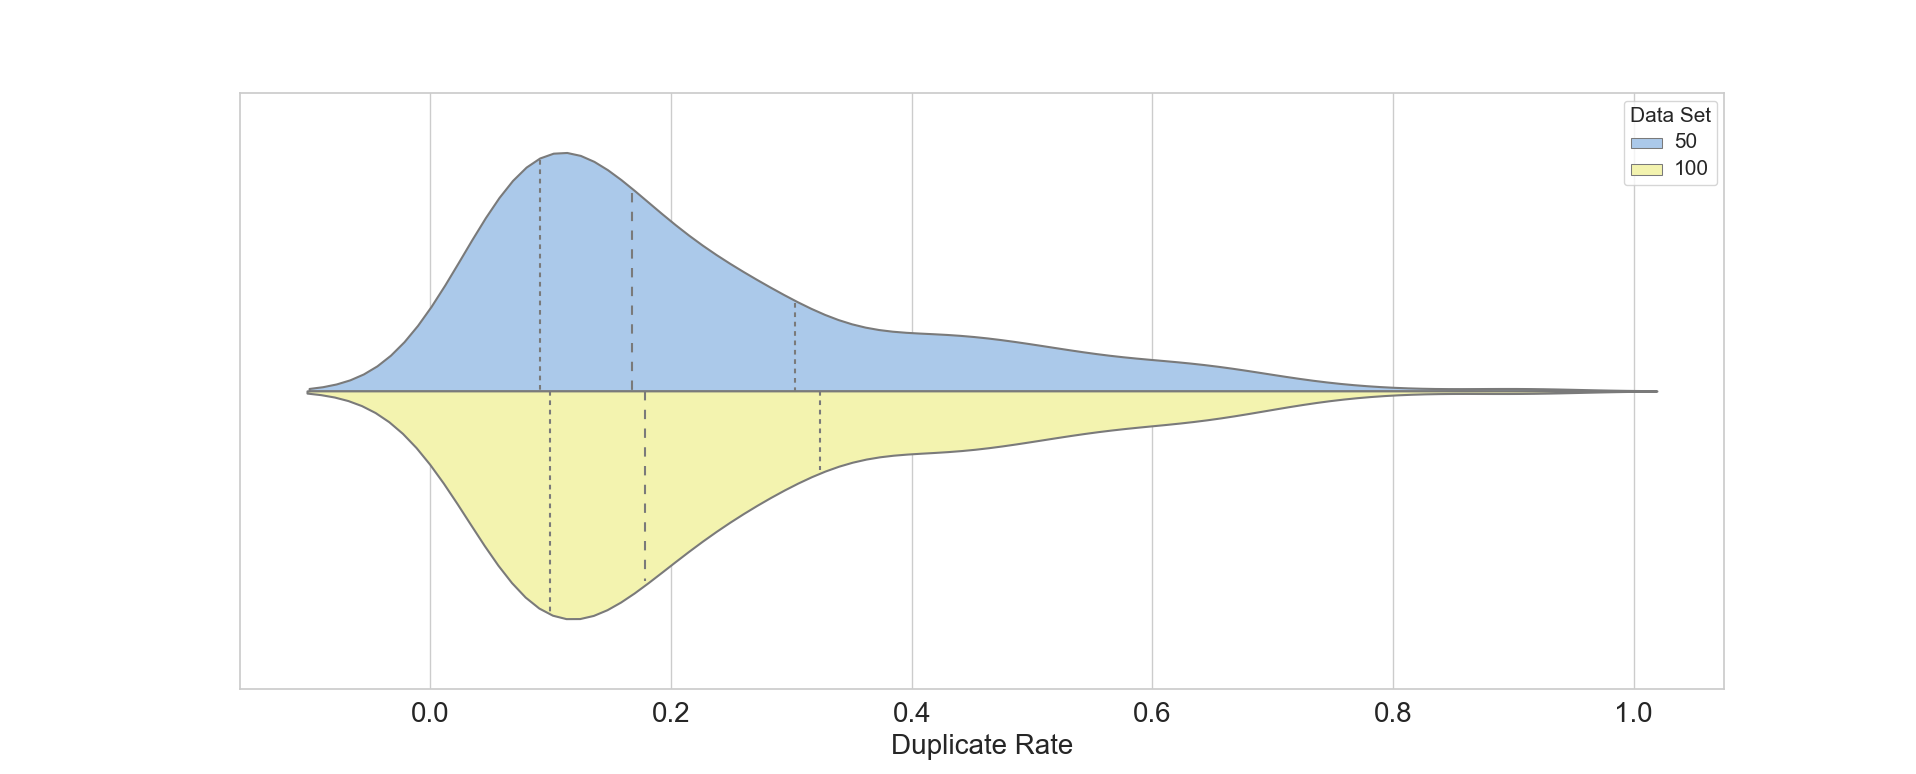
\includegraphics[width=\textwidth]{./Figures/edwin-cmt-simi-dist.png}
    \caption{两种数据组的应用评论重合率结果}
    \label{fig:cmt_simi}
\end{figure}

\begin{table}[htbp]
	\renewcommand{\arraystretch}{1}
	\small
	\centering
	\caption{评论重合率结果}
	\vspace{1mm}
	\begin{tabular}{lcccc}
		\toprule
		包名 & 评论重合率(\%) & 排名(数据组``50'') & 排名(数据组``100'') \\
		\midrule
		com.arsenal.FunWeather & 47.11 & 58 & 57 \\
		\rowcolor{gray!15} com.jhwl.fjxa & 44.97 & 66 & 65 \\
		com.sscwap & 10.98 & 349 & 325 \\
		\bottomrule
	\end{tabular}
	\label{table:cmt-simi-res}
\end{table}

\autoref{table:cmt-simi-res}提供了三款仿冒应用的评论重合率和在两组数据中的排名情况。
在``50''数据组的511个应用中,\emph{com.arsenal.FunWeather}和\emph{com.jhwl.fjxa}分别排名58和66(前11\%和前13\%),而在``100''数据组的455个应用中,\emph{com.arsenal.FunWeather}和\emph{com.jhwl.fjxa}的排名是57和65(前13\%和前14\%),都算是比较靠前的位置。
而且,只看评论重合率,两款应用的数值都超过了44\%,相当于差不多每五条评论中就有两条十分类似的评论,这表明上述两款应用很有可能使用了排名欺诈。
至于\emph{com.sscwap}的排名则比较偏后,较低的重合率说明其好评比较多元化,使用排名欺诈服务的可能性比较低。
本研究会在后面一节对这些结果进行验证。

\subsection{人工复核}

最后,本研究对\emph{com.arsenal.FunWeather}、\emph{com.jhwl.fjxa}和\emph{com.sscwap}的评论了进行人工复核。
为了方便复核,作者对每个应用的评论都按内容进行了排序。

\begin{figure}[htbp]
	\centering
	\subfloat[\emph{com.jhwl.fjxa}部分评论\label{fig:cmt-sample-1}]{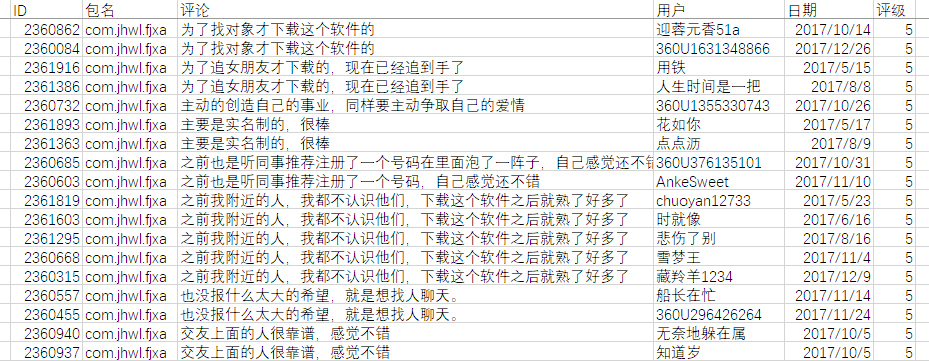
\includegraphics[width=\textwidth]{./Figures/edwin-cmt-sample-1.jpg}}\hfill

	\subfloat[\emph{com.arsenal.FunWeather}部分评论\label{fig:cmt-sample-2}]{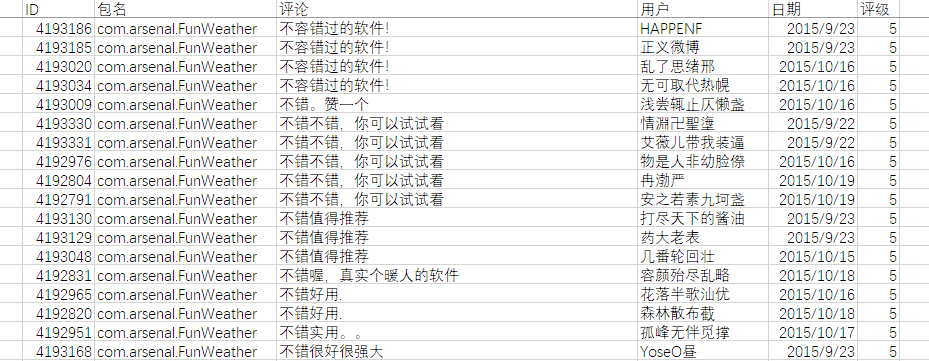
\includegraphics[width=\textwidth]{./Figures/edwin-cmt-sample-2.jpg}}\hfill

	\subfloat[\emph{com.sscwap}部分评论\label{fig:cmt-sample-3}]{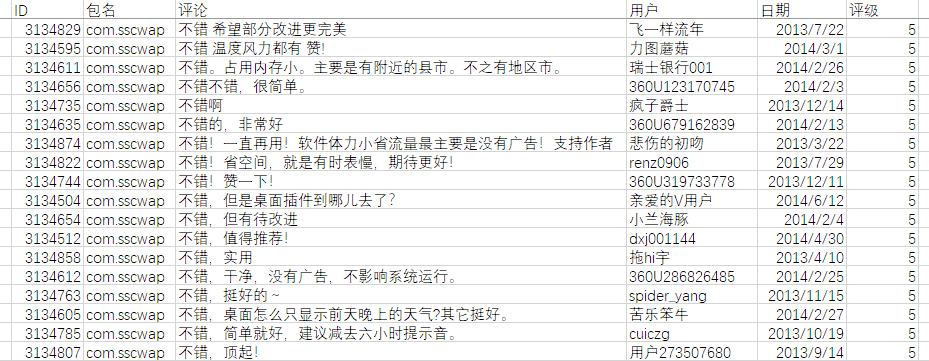
\includegraphics[width=\textwidth]{./Figures/edwin-cmt-sample-3.jpg}}\hfill
    \caption{应用评论取样}
    \label{fig:cmt-samples-1}
\end{figure}

\autoref{fig:cmt-samples-1}展示了本文对三款应用好评取样的结果。
可以明显看出,\emph{com.jhwl.fjxa}和\emph{com.arsenal.FunWeather}两款App都有明显的评论重复现象。
而图中对\emph{com.sscwap}的评论虽然看上去也比较近似,但这其实是由于本文按照评论内容对这些评论进行了一次排序。
如果结合日期数据观察,就能发现这些数据是由用户在比较分散的时间发出的。
所以说这些看上去稍微类似的评论,并不一定存在关联关系,作者不倾向于认为这款App购买了排名欺诈服务。
反观\autoref{fig:cmt-sample-1}中的评论,有多条长评论高度相似、甚至一模一样,这在真实案例中是不太可能会存在的情况;而\autoref{fig:cmt-sample-2}中多条近似、相同的评论是在十分接近的时间里被发表的,进一步加深了他们之间存在关联的可能性,所以本文十分有理由相信这两款应用的确存在排名欺诈的行为。

本研究还随机抽取了一些发布相同好评的不同用户进行追查,结果发现部分用户在研究收集到的数据集中的评论数只有一到两条,这很有可能是提供排名欺诈服务的商家规避检测的一种策略。

\section{本章小结}
本章从仿冒应用在市场中收到的评论入手,首先分析了用户对于这类应用的反响。
用户给出的反馈为一致好评,这十分出人意料。
进一步地,为验证仿冒应用与排名欺诈是否有关联,本文选取了部分应用的评论数据进行分析,并借鉴了前人研究提出了研究手段进行筛查。

一方面,从结果看,无论是基于评论内容相似度的排名欺诈排查方法还是基于用户可信度权重的排查方法,都证明了仿冒应用的确会利用排名欺诈服务提升自身的曝光率。
另一方面,用两种方法进行筛查也顺便比较了他们的有效性。
从性能层面看,两种方法有较大的区别。
研究发现,部分可疑好评的用户仅仅评论过一到两次,如果大部分排名欺诈用户都采用这种只发布少量好评的策略,基于用户可信度权重的排查方法就很可能会因为可参考的数据量太小而失效;
另外,基于用户可信度权重的排查方法会带来相当大的运算量,相比之下,基于评论内容相似度的代码只需几分钟就能运算完毕。
综合上述因素,本研究认为基于评论内容相似度的排查方法是更为可行的排查方式。
